\documentclass[letterpaper]{article}
%\documentclass[a5paper]{article}

%% Language and font encodings
\usepackage[english]{babel}
\usepackage[utf8x]{inputenc}
\usepackage[T1]{fontenc}

%% Sets page size and margins
\usepackage[letterpaper,top=.75in,bottom=1in,left=1in,right=1in,marginparwidth=1.75cm]{geometry}
%\usepackage[a5paper,top=1cm,bottom=1cm,left=1cm,right=1.5cm,marginparwidth=1.75cm]{geometry}

\usepackage{graphicx}
%\graphicspath{../images}	  %%where to look for images

%% Useful packages
\usepackage{amssymb, amsmath, amsthm} 
%\usepackage{graphicx}  %%this is currently enabled in the default document, so it is commented out here. 
\usepackage{calrsfs}
\usepackage{braket}
\usepackage{mathtools}
\usepackage{lipsum}
\usepackage{tikz}
\usetikzlibrary{cd}
\usepackage{verbatim}
%\usepackage{ntheorem}% for theorem-like environments
\usepackage{mdframed}%can make highlighted boxes of text
%Use case: https://tex.stackexchange.com/questions/46828/how-to-highlight-important-parts-with-a-gray-background
\usepackage{wrapfig}
\usepackage{centernot}
\usepackage{subcaption}%\begin{subfigure}{0.5\textwidth}
\usepackage{pgfplots}
\pgfplotsset{compat=1.13}
\usepackage[colorinlistoftodos]{todonotes}
\usepackage[colorlinks=true, allcolors=blue]{hyperref}
\usepackage{xfrac}					%to make slanted fractions \sfrac{numerator}{denominator}
\usepackage{enumitem}            
    %syntax: \begin{enumerate}[label=(\alph*)]
    %possible arguments: f \alph*, \Alph*, \arabic*, \roman* and \Roman*
\usetikzlibrary{arrows,shapes.geometric,fit}

\DeclareMathAlphabet{\pazocal}{OMS}{zplm}{m}{n}
%% Use \pazocal{letter} to typeset a letter in the other kind 
%%  of math calligraphic font. 

%% This puts the QED block at the end of each proof, the way I like it. 
\renewenvironment{proof}{{\bfseries Proof}}{\qed}
\makeatletter
\renewenvironment{proof}[1][\bfseries \proofname]{\par
  \pushQED{\qed}%
  \normalfont \topsep6\p@\@plus6\p@\relax
  \trivlist
  %\itemindent\normalparindent
  \item[\hskip\labelsep
        \scshape
    #1\@addpunct{}]\ignorespaces
}{%
  \popQED\endtrivlist\@endpefalse
}
\makeatother

%% This adds a \rewnewtheorem command, which enables me to override the settings for theorems contained in this document.
\makeatletter
\def\renewtheorem#1{%
  \expandafter\let\csname#1\endcsname\relax
  \expandafter\let\csname c@#1\endcsname\relax
  \gdef\renewtheorem@envname{#1}
  \renewtheorem@secpar
}
\def\renewtheorem@secpar{\@ifnextchar[{\renewtheorem@numberedlike}{\renewtheorem@nonumberedlike}}
\def\renewtheorem@numberedlike[#1]#2{\newtheorem{\renewtheorem@envname}[#1]{#2}}
\def\renewtheorem@nonumberedlike#1{  
\def\renewtheorem@caption{#1}
\edef\renewtheorem@nowithin{\noexpand\newtheorem{\renewtheorem@envname}{\renewtheorem@caption}}
\renewtheorem@thirdpar
}
\def\renewtheorem@thirdpar{\@ifnextchar[{\renewtheorem@within}{\renewtheorem@nowithin}}
\def\renewtheorem@within[#1]{\renewtheorem@nowithin[#1]}
\makeatother

%% This makes theorems and definitions with names show up in bold, the way I like it. 
\makeatletter
\def\th@plain{%
  \thm@notefont{}% same as heading font
  \itshape % body font
}
\def\th@definition{%
  \thm@notefont{}% same as heading font
  \normalfont % body font
}
\makeatother

%===============================================
%==============Shortcut Commands================
%===============================================
\newcommand{\ds}{\displaystyle}
\newcommand{\B}{\mathcal{B}}
\newcommand{\C}{\mathbb{C}}
\newcommand{\F}{\mathbb{F}}
\newcommand{\N}{\mathbb{N}}
\newcommand{\R}{\mathbb{R}}
\newcommand{\Q}{\mathbb{Q}}
\newcommand{\T}{\mathcal{T}}
\newcommand{\Z}{\mathbb{Z}}
\renewcommand\qedsymbol{$\blacksquare$}
\newcommand{\qedwhite}{\hfill\ensuremath{\square}}
\newcommand*\conj[1]{\overline{#1}}
\newcommand*\closure[1]{\overline{#1}}
\newcommand*\mean[1]{\overline{#1}}
%\newcommand{\inner}[1]{\left< #1 \right>}
\newcommand{\inner}[2]{\left< #1, #2 \right>}
\newcommand{\powerset}[1]{\pazocal{P}(#1)}
%% Use \pazocal{letter} to typeset a letter in the other kind 
%%  of math calligraphic font. 
\newcommand{\cardinality}[1]{\left| #1 \right|}
\newcommand{\domain}[1]{\mathcal{D}(#1)}
\newcommand{\image}{\text{Im}}
\newcommand{\inv}[1]{#1^{-1}}
\newcommand{\preimage}[2]{#1^{-1}\left(#2\right)}
\newcommand{\script}[1]{\mathcal{#1}}


\newenvironment{highlight}{\begin{mdframed}[backgroundcolor=gray!20]}{\end{mdframed}}

\DeclarePairedDelimiter\ceil{\lceil}{\rceil}
\DeclarePairedDelimiter\floor{\lfloor}{\rfloor}

%===============================================
%===============My Tikz Commands================
%===============================================
\newcommand{\drawsquiggle}[1]{\draw[shift={(#1,0)}] (.005,.05) -- (-.005,.02) -- (.005,-.02) -- (-.005,-.05);}
\newcommand{\drawpoint}[2]{\draw[*-*] (#1,0.01) node[below, shift={(0,-.2)}] {#2};}
\newcommand{\drawopoint}[2]{\draw[o-o] (#1,0.01) node[below, shift={(0,-.2)}] {#2};}
\newcommand{\drawlpoint}[2]{\draw (#1,0.02) -- (#1,-0.02) node[below] {#2};}
\newcommand{\drawlbrack}[2]{\draw (#1+.01,0.02) --(#1,0.02) -- (#1,-0.02) -- (#1+.01,-0.02) node[below, shift={(-.01,0)}] {#2};}
\newcommand{\drawrbrack}[2]{\draw (#1-.01,0.02) --(#1,0.02) -- (#1,-0.02) -- (#1-.01,-0.02) node[below, shift={(+.01,0)}] {#2};}

%***********************************************
%**************Start of Document****************
%***********************************************

%===============================================
%===============Theorem Styles==================
%===============================================

%================Default Style==================
\theoremstyle{plain}% is the default. it sets the text in italic and adds extra space above and below the \newtheorems listed below it in the input. it is recommended for theorems, corollaries, lemmas, propositions, conjectures, criteria, and (possibly; depends on the subject area) algorithms.
\newtheorem{theorem}{Theorem}
\numberwithin{theorem}{section} %This sets the numbering system for theorems to number them down to the {argument} level. I have it set to number down to the {section} level right now.
\newtheorem*{theorem*}{Theorem} %Theorem with no numbering
\newtheorem{corollary}[theorem]{Corollary}
\newtheorem*{corollary*}{Corollary}
\newtheorem{conjecture}[theorem]{Conjecture}
\newtheorem{lemma}[theorem]{Lemma}
\newtheorem*{lemma*}{Lemma}
\newtheorem{proposition}[theorem]{Proposition}
\newtheorem*{proposition*}{Proposition}
\newtheorem{problemstatement}[theorem]{Problem Statement}


%==============Definition Style=================
\theoremstyle{definition}% adds extra space above and below, but sets the text in roman. it is recommended for definitions, conditions, problems, and examples; i've alse seen it used for exercises.
\newtheorem{definition}[theorem]{Definition}
\newtheorem*{definition*}{Definition}
\newtheorem{condition}[theorem]{Condition}
\newtheorem{problem}[theorem]{Problem}
\newtheorem{example}[theorem]{Example}
\newtheorem*{example*}{Example}
\newtheorem*{counterexample*}{Counterexample}
\newtheorem*{romantheorem*}{Theorem} %Theorem with no numbering
\newtheorem{exercise}{Exercise}
\numberwithin{exercise}{section}
\newtheorem{algorithm}[theorem]{Algorithm}

%================Remark Style===================
\theoremstyle{remark}% is set in roman, with no additional space above or below. it is recommended for remarks, notes, notation, claims, summaries, acknowledgments, cases, and conclusions.
\newtheorem{remark}[theorem]{Remark}
\newtheorem*{remark*}{Remark}
\newtheorem{notation}[theorem]{Notation}
\newtheorem*{notation*}{Notation}
%\newtheorem{claim}[theorem]{Claim}  %%use this if you ever want claims to be numbered
\newtheorem*{claim}{Claim}



\pgfplotsset{compat=1.13}

%\newcommand{\T}{\mathcal{T}}
%\newcommand{\B}{\mathcal{B}}
\newcommand{\arbcup}[1]{\bigcup\limits_{\alpha\in\Gamma}#1_\alpha}
\newcommand{\arbcap}[1]{\bigcap\limits_{\alpha\in\Gamma}#1_\alpha}
\newcommand{\Rbad}{\R_\text{bad}}

\title{Math 501 \linebreak
Homework 10}
\author{Trevor Klar}

\begin{document}

\maketitle

\begin{enumerate}
\item Which of the following are connected? Justify your answer. 
	\begin{enumerate}
	\item $\R^1_\text{bad}$
	\begin{proof}[Answer:]
	Not connected, since $[-\infty,0)\cup [0,\infty)$ is a separation of $\R^1_\text{bad}$. Also, every set in this topology is both closed and open (clopen), which also proves the space is not connected. 
	\end{proof}
	
	\item $\R^1_\text{finite complement}$
	\begin{proof}[Answer:]
	Connected. No two nonempty open sets are disjoint, so they cannot separate the space. Also, every closed sets has a greatest element, so no two closed sets can cover the whole space. Furthermore, since the space is infinite, no closed set (besides $\R^1_\text{finite complement}$) can have a finite complement, so the only clopen sets are $\emptyset$ and $\R^1_\text{finite complement}$. 
	\end{proof}
	
	\item The set of all points in $\R^2$ with at least one coordinate a rational number. 
	
	\begin{proof}[Answer:]
	Connected. Let $S$ denote the whole set, and consider the following subsets of $S$:
	\[\begin{array}{c}
	\Q\times\R = \{(q,r)\in\R^2 : q\in\Q, r\in\R \}\\
	\R\times\Q = \{(r,q)\in\R^2 : r\in\R, q\in\Q \}\\
	\Q\times\Q = \{(q_1,q_2)\in\R^2 : q_1,q_2\in\Q \}\\
	\end{array}\]
	First, note that $\Q\times\Q \subset \left(\Q\times\R\cup \R\times\Q \right)=S$. Also note that for any $q\in\Q$, we have that 
	$$\{q\}\times\R \quad \cong \quad \R \quad \cong \quad \R\times\{q\},$$
	 so any set of one of those forms is connected. As a final preliminary observation, note that $\left\lbrace\R \times \{q\} : q\in\Q\right\rbrace = \R\times\Q$, and $\left\lbrace \{q\}\times\R : q\in\Q \right\rbrace = \Q\times\R$.
	 
	 Now, consider $(\{1\}\times\R)$. For every $q_1\in\Q$, we can see that $(\{1\}\times\R) \cap (\R\times\{q_1\}) = (1,q_1)$, so $(\{1\}\times\R) \cup (\R\times\Q)$ is connected by Theorem 45. 

	\begin{center}
	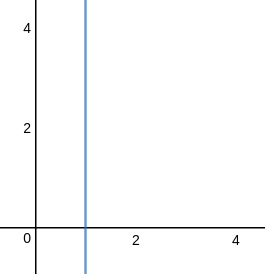
\includegraphics[scale=.3]{hw10_prob1c_1}
	\quad
	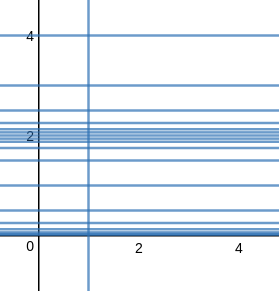
\includegraphics[scale=.3]{hw10_prob1c_2}
	\end{center}
	 
	 Second, consider $(\R\times\{1\})$. For every $q_2\in\Q$, we can see that $(q_2\times\R) \cap (\R\times\{1\}) = (q_2,1)$, so $(\Q\times\R) \cup (\R\times\{1\})$ is connected by Theorem 45. 
	 
	\begin{center}
	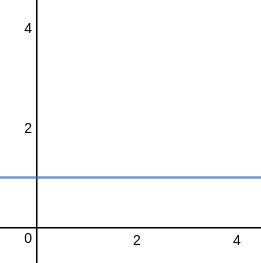
\includegraphics[scale=.3]{hw10_prob1c_3}
	\quad
	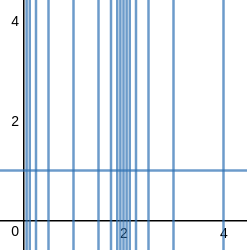
\includegraphics[scale=.3]{hw10_prob1c_4}
	\end{center}
	 
	 Finally, note that $(1,1)\in ((\{1\}\times\R) \cup (\R\times\Q)) \cap ((\Q\times\R) \cup (\R\times\{1\})) = \left(\Q\times\R\cup \R\times\Q \right)=S$, so $S$ is connected, and we are done. 
	 
	\begin{center}
	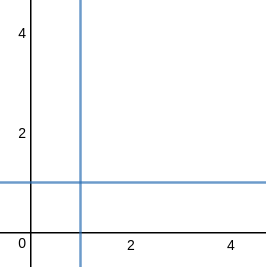
\includegraphics[scale=.3]{hw10_prob1c_5}
	\quad
	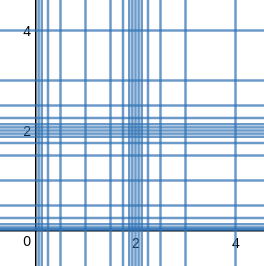
\includegraphics[scale=.3]{hw10_prob1c_6}
	\end{center}
	 
	\end{proof}
	
	\item The set of all points in $\R^2$ with both coordinates a rational number. 
	\begin{proof}[Answer:]
	Not connected, since the rational half-planes $$\{(x,y)\in\Q^2 : x<\pi)\}\cup\{(x,y)\in\Q^2 : x>\pi)\}$$ form a separation for the set. To see this, note that the two sets are open in $\Q^2$ (with the subspace topology in $\R^2$), they are disjoint, and their union is $\Q^2$, the set in question. 
	\end{proof}
	
	\end{enumerate}

\item Use the connectedness of $[a,b]$ to prove the Intermediate Value Theorem: If $f:[a,b]\to\R$ is a continuous function with $f(a)>0$ and $f(b)<0$, then there exists $c\in(a,b)$ with $f(c)=0$. 
\begin{proof}
Let $f$ be a function as described above. Since $(-\infty,0)$ and $(0,\infty)$ are disjoint and open in $\R$ and $f$ is continuous, then 
$$\preimage{f}{(-\infty,0)} \text{ and } \preimage{f}{(0,\infty)}$$ 
are also disjoint and open in $[a,b]$. Now, since $f(a)>0$ and $f(b)<0$, then $a\in\preimage{f}{(0,\infty)}$ and $b\in\preimage{f}{(-\infty,0)}$. Now we have that $\preimage{f}{(-\infty,0)}$ and $\preimage{f}{(0,\infty)}$ are nonempty, disjoint, open sets in $[a,b]$. Since $[a,b]$ is connected, 
$$\preimage{f}{(-\infty,0)} \cup \preimage{f}{(0,\infty)} \neq [a,b],$$ 
because otherwise the two sets would comprise a separation of $[a,b]$. Now, we have already considered the preimage of the entire target space, except the singleton $\{0\}$. This means that $\preimage{f}{\{0\}}\neq\emptyset$, which is to say that there exists $c\in(a,b)$ with $f(c)=0$. 
\end{proof}

\item Let $X$ be a connected metric space with an unbounded metric $d$. Prove that every sphere $S(x_0,r)=\{x:d(x_0,x)=r\}$ is nonempty. 
\begin{proof}
Let $r>0$ be any nonzero real number. Consider the following sets:
$$B(x_0,r)\cup\closure{B}^\complement(x_0,r).$$
All following balls will have the same center and radius, so we will omit that notation for brevity. Now, we know already that open balls are open sets, so $B$ is open. Since its closure $\closure{B}$ is of course closed, then $\closure{B}^\complement$ is open. Since $B\subset\closure{B}$, then $B$ and $\closure{B}^\complement$ are disjoint. Now $d$ is a metric, and so is positive definite, which means $d(x_0,x_0)=0$; so $x_0\in B$. Also, $d$ is an unbounded metric, so there exists some $x'\in X$ such that $d(x_0,x')>r$, which means $x'\in\closure{B}^\complement$. Therefore, $B$ and $\closure{B}^\complement$ are nonempty, open, disjoint sets in $X$, so $B \cup \closure{B}^\complement \subsetneq X$ (Otherwise, they would comprise a separation of $X$, which contradicts that $X$ is connected). Since 
$$B \cup \closure{B}^\complement = \{x:d(x_0,x)<r \text{ or } d(x_0,x)>r \},$$
then $S(x_0,r)=\{x:d(x_0,x)=r\}$ is nonempty.
\end{proof}

\pagebreak
\item Prove Proposition 43: Suppose that $A$ is a connected subset of $X$. If $B$ is a subset of $X$ such that $A\subset B\subset \closure{A}$, then $B$ is connected. 
\begin{proof}
Suppose that $A$ is a connected subset of $X$, and $B$ is a subset of $X$ such that $A\subset B\subset \closure{A}$. Since $\closure{A}-A\subset A^\ell$ and $B-A\subset A^\ell$, it suffices to show that for any $a\in A^\ell$, $A\cup\{a\}$ is connected. 

Let $a\in A^\ell$. Suppose for contradiction that $U\cup C$ is a separation of $A\cup\{a\}$. Now, $a\in U$ or $a\in V$, since otherwise $U\cup V \neq (A\cup\{a\})$. So without loss of generality, let $a\in U$. Since $U\cup V = (A\cup\{a\})$, then $(U-\{a\}\cup V = A)$ is a separation of $A$, which contradicts that $A$ is connected. Thus, $A\cup\{a\}$ is connected. 

To see that we are done, note that 
$$\bigcup_{b\in B-A}(\{b\} \cup A) = B,$$
and each $\{b\} \cup A$ was shown to be connected above, and they all have the elements of $A$ in common. Similarly, $\bigcup_{a\in \closure{A}-A}(\{a\} \cup A) = \closure{A}$ is connected for the same reason. 
\end{proof}

\item Prove that $[0,1]$, $[0,\infty)$, $S^1$, and $\R$ are pairwise not homeomorphic. 

\begin{lemma*}
Let $X$, $Y$ be connected sets. If $X\cong Y$, then for any point $x\in X$ such that $X-\{x\}$ is connected, there exists a point $y\in Y$ such that $Y-\{y\}$ is connected. 
\end{lemma*}
\begin{proof} Suppose $X\cong Y$ with homeomorphism $f:X\to Y$, and let $x\in X$ be a point such that $X-\{x\}$ is connected. Suppose for contradiction that for any point $y\in Y$, we have that that $Y-\{y\}$ is not connected. Fix $y=f(x)$, and let $U\cup V$ be a separation of $Y-\{y\}$. Now consider $\preimage{f}{U}$ and $\preimage{f}{V}$. Since $f$ is a continuous function, $\preimage{f}{U}$ and $\preimage{f}{V}$ are disjoint open sets which cover $X-\{x\}$, so they are a separation of $X-\{x\}$. This contradicts our assumption that $X-\{x\}$ is connected, so we conclude that there exists a point $y\in Y$ such that $Y-\{y\}$ is connected.
\end{proof}

\begin{corollary*}
Let $X$, $Y$ be connected sets. $X\cong Y$ if and only if for any point $x\in X$ such that $X-\{x\}$ is \emph{not} connected, there exists a point $y\in Y$ such that $Y-\{y\}$ is \emph{not} connected. 
\end{corollary*}
\begin{proof}
Suppose $X\cong Y$ with homeomorphism $f:X\to Y$, and let $x\in X$ be a point such that $X-\{x\}$ is not connected. Suppose for contradiction that for any point $y\in Y$, we have that that $Y-\{y\}$ is connected. Since $f$ is a homeomorphism, it has an inverse $F:Y\to X$. Fix $y=f(x)$ and let $U\cup V$ be a separation of $X-\{x\}$. Now consider $\preimage{F}{U}$ and $\preimage{F}{V}$. By the same reasoning as in the Lemma, $\preimage{F}{U} \cup \preimage{F}{V}$ is a separation of $Y-\{y\}$, so there exists a point $y\in Y$ such that $Y-\{y\}$ is not connected.
\end{proof}

\begin{proof}\textbf{of Problem 5}
All of these sets are subsets of the real numbers, and since $[0,1]$ and $S^1$ are closed and bounded, then they are compact by the Heine-Borel Theorem. We have already proven that the other two sets are not compact. Now, none of the compact sets are homeomorphic the the noncompact sets, and vice versa. So it suffices to show that $[0,\infty)\not\cong\R$ and $[0,1]\not\cong S^1$.  

Note that $[0,\infty)-\{0\}$ is connected. However, $\R-\{x\}$ is not connected for any $x\in\R$. Thus, by the contrapositive of the Lemma, $[0,\infty)\not\cong\R$.

Also note that $[0,1]-\{\sfrac{1}{2}\}$ is not connected. However, for any point $p\in S^1$, $S^1-\{p\}$ is connected. Thus, by the contrapositive of the Corollary, $[0,1]\not\cong S^1$. 
%\begin{center}
%\begin{tabular}{c|c|c|c}
%$[0,1]$ & $[0,\infty)$ & $S^1$ & $\R$\\
%\hline
%Compact & Not compact & Compact & Not compact\\
%Not open & Not open & Not open & Open \\
%Closed & Not closed & Closed & Closed \\
%\end{tabular}
%\end{center}
\end{proof}

\item TRUE or FALSE? If $A$ is a path-connected subset of $X$, and $B$ is a subset of $X$ such that $A\subset B\subset \closure{A}$, then $B$ is path-connected. Prove or give a counterexample. 
\begin{proof}[\textbf{Counterexample}] Consider the folowing sets:
\[\begin{array}{rl}
G_f=A=&\left\lbrace\left(x,\sin \tfrac{1}{x}\right) : x \in (0,\infty)\right\rbrace\\
\closure{G_f}=B=&\left\lbrace\left(x,\sin \tfrac{1}{x}\right) : x \in (0,\infty)\right\rbrace \cup \{(0,y) : -1\leq y\leq 1 \}\\
\end{array}\]
$G_f$ is path connected by construction, since it is defined by the functions $x$ and $\sin \tfrac{1}{x}$, which are continuous on the open interval $(0,\infty)$. We have already shown in class that $\closure{G_f}$ is not path connected because there are no paths connecting points in $\left\lbrace\left(x,\sin \tfrac{1}{x}\right) : x \in (0,\infty)\right\rbrace$ to points in $\{(0,y) : -1\leq y\leq 1 \}$, so we are done.
\end{proof}

\end{enumerate}

\end{document}
